%!TEX root = ../main.tex

\chapter{Symbolic-Numerical Analysis and Solution of Structures}
\label{app4:trussme}

Understanding how structures react to external forces and imposed displacements relies heavily on structural mechanics. Typically, structural analysis is carried out numerically using the direct stiffness method, a finite element method implementation known for solving large systems of equations. However, this method's principles can also be applied symbolically or in a hybrid symbolic-numerical manner for structural analysis. This dual approach is valuable for reducing computational load, as symbolic solutions can be simplified and translated into efficient code for simulations. Moreover, symbolic direct stiffness methods facilitate model reduction, enabling the creation of smaller-scale models for faster simulations. Despite its advantages, symbolic computation has limitations, particularly in solving large linear systems of equations, which can be computationally intensive and may exceed software capabilities. This chapter introduces \TrussMe{}, a toolbox built on the direct stiffness method, harnessing symbolic computation from \Maple{} and numerical capabilities from \Matlab{} for structural analysis. The toolbox facilitates both symbolic and hybrid symbolic-numerical analyses, streamlining code generation for efficient simulations. To address challenges in solving large linear systems symbolically, \TrussMe{} incorporates novel routines for symbolic matrix factorization, employing hierarchical representation for managing large expressions. Optionally, the toolbox integrates with \LEM{} and \LAST{}, open-source \Maple{} packages, enhancing its symbolic computation capabilities.

% % % % % % % % % % % % % % % % % % % % % % % % % % % % % % % % % % % % % % % %

\section{Introduction to Symbolic Structural Analysis}
\label{app4:sec:introduction}

Structural mechanics is foundational in engineering for predicting system behavior under external forces. Achieving optimal performance in mechanical systems requires refining analytical processes to ensure precision and reliability, especially with the increasing adoption of complex structures. Structural analysis typically involves evaluating deformations and internal reactions under specified boundary conditions (\acp{BC}), such as applied loads and displacements. Accurately predicting these responses is crucial for identifying critical areas and optimizing performance during the design process. Moreover, it is essential for simulating dynamic behavior during the simulation phase.

Traditionally, deformation and internal reaction analysis are performed numerically using the Finite Element Method (\ac{FEM}), which was introduced in the mid-20th century and is now widely utilized for analyzing complex structures with relative ease \cite{felippa2001historical}. It's important to note that \ac{FEM} is a general concept based on discretizing structures into finite elements, leading to multiple implementation approaches with varying performance and capabilities across software platforms. Specifically, the \ac{FEM} implementation used in this chapter is the \ac{DSM}, introduced by Turner in 1959 \cite{turner1959direct} and further refined in 1964 \cite{turner1964further}. DSM involves assembling stiffness matrices of individual elements into a global stiffness matrix, which is then used to solve equations relating node displacements and rotations to internal and external forces and moments. \acp{BC} are enforced by appropriately modifying the global stiffness matrix, force, and displacement vectors. Consequently, DSM is a versatile method applicable to various structures, including trusses, beams, frames, and plates.

The drive to optimize product performance while minimizing design and production costs necessitates parametric studies and optimization techniques. However, traditional numeric design optimization brings complexities, requiring numerous simulations and substantial computational resources. In response, symbolic computation emerges as a valuable alternative. While the \ac{DSM} is typically associated with numerically solving large equation systems, its theoretical underpinning enables symbolic or hybrid symbolic-numerical structural analysis. Symbolic solutions provide crucial derivatives of the solution concerning structural parameters, essential for optimization. Additionally, symbolic approaches facilitate lean code generation, exploiting expression simplification for efficient simulations. Symbolic \ac{DSM} also aids model reduction by deriving smaller models to reduce simulation time. Despite its advantages, symbolic computation poses challenges, particularly in solving large linear equation systems due to software limitations \cite{carette2006linear, zhou2007symbolic}.

Symbolic computation in structural analysis has been explored in literature \cite{noor1979computerized, pavlovic2003symbolic}. Successful attempts include symbolic manipulation in stiffness matrix generation \cite{cecchi1977automatic} and solving equation systems \cite{ioakimidis1992application, beltzer2012variational}. However, as highlighted in \cite{pavlovic2003symbolic}, symbolic structural solution remains limited by symbolic kernel capabilities, restricting analysis to relatively small structures. Nonetheless, recent decades have seen significant advancements in solving large linear equation systems symbolically \cite{carette2006linear, zhou2007symbolic}. These advances, utilizing symbolic matrix factorization with hierarchical representation, enable solutions previously deemed impractical.

The absence of a symbolic analysis and solution package for structures within the \Maple{} environment spurred the development of this toolbox\footnote{It is worth noting that, unlike \Maple{}, \Mathematica{} features a pre-existing suite of packages tailored for symbolic analysis of elastic structural elements, known as the \emph{Structural Mechanics} package~\cite{structuralmechanics}.}. Specifically, the authors' necessity for a tool to symbolically represent, solve, and generate code for modeling, simulating, and optimizing compliant mechanisms prompted the creation of \TrussMe{}. Leveraging the symbolic computation capabilities of \Maple{} and the numerical prowess of \Matlab{}, this toolbox constructs a framework for symbolic-numerical analysis and solution of structures. Grounded in the aforementioned \ac{DSM}, the solution method enables modeling, analysis, and resolution of structures. Depending on the symbolic kernel's capabilities, available computation time, and problem complexity, the symbolic solution can manifest either symbolically in closed form or numerically. In either scenario, a \Matlab{} class is generated to efficiently assess the symbolic solution or solve the problem numerically. Throughout code generation, model inputs and class internal data are meticulously mapped to the generated code. Particular emphasis is placed on the symbolic solution of linear equation systems stemming from the \ac{DSM}. Novel symbolic routines, extending both built-in \Maple{} routines and prior works such as \cite{carette2006linear, zhou2007symbolic}, are introduced to conduct symbolic matrix factorization (\LAST{}~\cite{last}) with hierarchical representation of large expressions (\LEM{}~\cite{lem}). This expansion broadens the applicability of symbolic solution to larger structures previously deemed infeasible. The toolbox, named \TrussMe{}, along with its optional dependencies, is released as open-source software under the BSD 3-clause license~\cite{trussme}.

%The chapter's structure is as follows: Following the introduction (Section~\ref{app4:sec:introduction}), we offer a concise overview of the \ac{DSM} and the solution method utilized by the toolbox (Section~\ref{app4:sec:solution_method}). Section~\ref{app4:sec:software_description} delineates the toolbox's implementation, dependencies, and usage. An illustrative example of the toolbox's application to optimization, modeling, and simulation of a complex mechanism is presented in Section~\ref{app4:sec:example_applications}. Finally, concluding remarks are provided in Section~\ref{app4:sec:conclusion}.

% % % % % % % % % % % % % % % % % % % % % % % % % % % % % % % % % % % % % % % %

\section{The Direct Stiffness Method}
\label{app4:sec:solution_method}

The forthcoming elucidation of the solution method is indispensable for grasping the toolbox implementation and is not intended to offer an exhaustive review of the \ac{DSM}. For a more thorough understanding of \ac{DSM} theory, please consult~\cite{turner1959direct, turner1964further, logan2002first, hutton2004fundamentals}. As delineated in~\cite{samuelsson2006history}, \ac{DSM} furnishes a systematic approach to analyzing statically determinate and indeterminate structures. The structural analysis problem can be formulated as follows: given a structure subjected to external loads and/or prescribed displacements, determine the displacements and rotations of the nodes, along with the internal forces and moments within the elements. These displacements and rotations of nodes are termed Degrees of Freedom (\acp{DOF}). The relationship between \acp{DOF} and the forces and moments acting on the structure—both internal and external—is encapsulated in the system of equations
%
\begin{equation}
  \label{app4:eq:system}
  \mathbf{K}^{n} \, \mathbf{d}^{n} = \mathbf{f}^{n}.
\end{equation}
%
Here, $\mathbf{K}^{n} \in \mathbb{R}^{N \times N}$ represents the stiffness matrix, $\mathbf{d}^{n} \in \mathbb{R}^{N}$ denotes the displacement vector, $\mathbf{f}^{n} \in \mathbb{R}^{N}$ signifies the force vector, and $N$ signifies the number of Degrees of Freedom (\acp{DOF}) of the structure. The superscript $n$ indicates that these quantities are expressed in the nodes' reference frames. Subsequent sections briefly outline the derivation of the components of the system of equations~\eqref{app4:eq:system}. Furthermore, the toolbox's solution method for effectively handling the system of equations is elucidated.

\subsection{Element Stiffness Matrix}

To derive the global stiffness matrix $\mathbf{K}^{n}$ in~\eqref{app4:eq:system}, we must initially define the stiffness matrix $\Ke \in \mathbb{R}^{\Ne \times \Ne}$ for individual elements $e \in \mathcal{E}$, which connect a subset of the structure's nodes. Here, $\mathcal{E}$ denotes the set of elements in the structure, and $\Ne$ signifies the number of Degrees of Freedom (\acp{DOF}) of the element. Unless specified otherwise, the matrix $\Ke$ is always assumed to be expressed in the element reference frame. Stiffness matrices are derived from various theories, such as the Euler-Bernoulli and the Timoshenko-Ehrenfest beam theories, the plane stress theory, etc.~\cite{hutton2004fundamentals}. However, describing the derivation of such matrices $\Ke$ is beyond our scope,
%of this work,
and they are assumed to be known.

\subsection{Element Stiffness Matrix Condensation}

The stiffness matrix $\Ke$ delineates how an element reacts when subjected to unit displacements imposed at each of its nodes' Degrees of Freedom (\acp{DOF}). Typically, when deriving such a matrix, it is assumed that the element is rigidly connected at each of its nodes' \acp{DOF}, thus possessing no internal \acp{DOF}. However, in certain structures, internal \acp{DOF} may arise due to links that permit specific movements at nodes while constraining others. To address this scenario, the matrix $\Ke$ must be adjusted accordingly~\cite{logan2002first}. This adjustment, known as \emph{condensation}, involves reordering rows and columns of the matrix $\Ke$ such that rows and columns corresponding to free nodal \acp{DOF} are relocated to the bottom-right corner of the matrix. This reordering, executed via a permutation matrix $\Pe$, facilitates the elimination of stiffness entries associated with free nodal \acp{DOF} from the original matrix $\Ke$. Consequently, a new condensed stiffness matrix ${\Ke}_{,c} \in \mathbb{R}^{{\Ne}_{,c} \times {\Ne}_{,c}}$ is derived, where ${\Ne}_{,c}$ denotes the number of constrained \acp{DOF} of the element. The condensed stiffness matrix ${\Ke}_{,c}$ is then computed through the following operations
%
\begin{equation}
  \Pe \, \Ke \, \Pe^\top= \left[\,\begin{matrix}
    {\Ke}_{,11} & {\Ke}_{,12} \\[0.5em]
    {\Ke}_{,21} & {\Ke}_{,22}
  \end{matrix}\,\right] \quad \xrightarrow[\text{condensation}]{\text{stiffness}} \quad
   \Pe \, {\Ke}_{,c} \, \Pe^\top = \left[\,\begin{matrix}
    {\Ke}_{,11} - {\Ke}_{,12} \, {{\Ke}_{,22}}^{-1} \, {\Ke}_{,21} & 0 \\[0.5em]
    0 & 0
  \end{matrix}\,\right] \text{.}
\end{equation}
%
It's important to apply condensation to each element of the structure as needed. Subsequently, the subscript $c$ in ${\Ke}_{,c}$ is dropped, and the condensed stiffness matrix is denoted simply as $\Ke$.

\subsection{Global Stiffness Matrix Assemblage}

The global stiffness matrix $\mathbf{K}^{g}$ is constructed by aggregating the stiffness contributions from individual elements of the structure. The superscript $g$ signifies that these quantities are expressed in the global reference frame. To achieve this, the element's stiffness matrix $\Ke^{g}$ is initially derived by transforming $\Ke$ from the element reference frame to the global reference frame as follows
%
\begin{equation}
  \label{app4:eq:element_stiffness_matrix}
  \Ke^{g} = \Te^\top \, \Ke \, \Te \text{,} \qquad \text{where} \qquad \Te = \left[\,\begin{matrix}
    \Re    & \ldots & 0 \\[0.25em]
    \vdots & \ddots & \vdots \\[0.25em]
    0      & \ldots & \Re
  \end{matrix}\,\right] \text{.}
\end{equation}
%
Note that $\Re$ represents the rotation matrix from the $e$-th element reference frame to the global reference frame. Each transformed stiffness matrix $\Ke^{g}$ is then integrated into the global stiffness matrix $\mathbf{K}^{g}$ by incorporating the contributions of individual elements into their respective positions corresponding to the structure's Degrees of Freedom (\acp{DOF}). Consequently, the matrix $\Ke^{g}$ is multiplied by the injection matrix $\Je \in \mathbb{R}^{\Ne \times N}$, which is a matrix consisting mainly of zeros except for the positions corresponding to the structure's \acp{DOF}, which are set to one. Thus, the global stiffness matrix $\mathbf{K}^{g}$ is formulated as follows
%
\begin{equation}
  \mathbf{K}^{g} = \sum_{e \, \in \, \mathcal{E}} \Je^\top \, \Ke^{g} \, \Je
   = \sum_{e \, \in \, \mathcal{E}} \Je^\top \, \Te^\top\,\Ke \, \Te \, \Je \text{,}
\end{equation}
%
where $\mathcal{E}$ is the set of elements of the structure.

Following this transformation, we arrive at the linear system of equations~\eqref{app4:eq:system} expressed in the global reference frame, denoted as $\mathbf{K}^{g} \, \mathbf{d}^{g} = \mathbf{f}^{g}$, where $\mathbf{d}^{g}$ and $\mathbf{f}^{g}$ represent the displacement and force vectors in the global reference frame, respectively. However, boundary conditions (\acp{BC}) for displacements and forces are typically applied in the nodes' reference frames. Consequently, to account for this, the system of equations~\eqref{app4:eq:system} must be adjusted by incorporating the nodes' rotations $\mathbf{Q}_{i}$ with respect to the global reference frame, which are consolidated in the block diagonal matrix $\mathbf{Q}$. This adjustment allows us to express the system~\eqref{app4:eq:system} as
%
\begin{equation}
  \underbrace{\mathbf{Q} \, \mathbf{K}^{g} \, \mathbf{Q}^\top}_{\displaystyle\mathbf{K}^{n}} \, \underbrace{\mathbf{Q} \, \mathbf{d}^{g}}_{\displaystyle\mathbf{d}^{n}} = \underbrace{\mathbf{Q} \, \mathbf{f}^{g}}_{\displaystyle\mathbf{f}^{n}} \text{,} \qquad \text{where} \qquad \mathbf{Q} = \left[\,\begin{matrix}
    \mathbf{Q}_{1} & \ldots & 0 \\[0.25em]
    \vdots       & \ddots & \vdots \\[0.25em]
    0            & \ldots & \mathbf{Q}_{\mathcal{N}}
  \end{matrix}\,\right] \text{,}
\end{equation}
%
and $\mathcal{N}$ is the number of nodes of the structure.

To construct the nodal force vector $\mathbf{f}^{n}$ and displacement vector $\mathbf{d}^{n}$, it's necessary to incorporate the individual nodes' boundary conditions (\acp{BC}) into their corresponding Degrees of Freedom (\acp{DOF}). This process involves multiplying the $i$-th nodal force vector $\mathbf{f}^{n}_{i}$ and displacement vector $\mathbf{d}^{n}_{i}$ by the injection matrix $\mathbf{J}_{i} \in \mathbb{R}^{N_i \times N}$, where $N_i$ represents the number of \acp{DOF} of the node. Consequently, the vectors $\mathbf{f}^{n}$ and $\mathbf{d}^{n}$ are derived as
%
\begin{equation}
  \mathbf{f}^{n} = \sum_{i \, \in \, \mathcal{N}} \mathbf{J}_{i}^\top \, \mathbf{f}^{n}_{i}
  \qquad \text{and} \qquad
  \mathbf{d}^{n} = \sum_{i \, \in \, \mathcal{N}} \mathbf{J}_{i}^\top \, \mathbf{d}^{n}_{i} \text{.}
\end{equation}

\subsection{Linear System Partitioning and Solution}

To solve the system of equations~\eqref{app4:eq:system}, it's beneficial to split it into two distinct sets of equations: the first set is solved for the free displacements $\mathbf{d}^{n}_{f}$, while the second set is solved for the reaction (internal) forces $\mathbf{f}^{n}_{s}$. This division is accomplished by rearranging and partitioning the stiffness matrix $\mathbf{K}^{n}$ into four submatrices $\mathbf{K}^{n}_{ff}$, $\mathbf{K}^{n}_{fs}$, $\mathbf{K}^{n}_{sf}$, and $\mathbf{K}^{n}_{ss}$, where the subscripts $f$ and $s$ denote the free and specified (or subject to \acp{BC}) Degrees of Freedom (\acp{DOF}), respectively. Similarly, the displacement and force vectors are partitioned accordingly, e.g., $\mathbf{d}^{n}_{f}$, $\mathbf{d}^{n}_{s}$, and $\mathbf{f}^{n}_{f}$, $\mathbf{f}^{n}_{s}$. Subsequently, the system of equations~\eqref{app4:eq:system} can be expressed as
%
\begin{equation}
    \label{app4:eq:macrofe}
    \underbrace{\left[\,\begin{matrix}
      \mathbf{K}^{n}_{ff} & \mathbf{K}^{n}_{fs} \\[0.5em]
      \mathbf{K}^{n}_{sf} & \mathbf{K}^{n}_{ss}
    \end{matrix}\,\right]}_{\displaystyle \mathbf{P}^{n} \, \mathbf{K}^{n} \, (\mathbf{P}^{n})^\top} \underbrace{\left[\,\begin{matrix}
      \mathbf{d}^{n}_{f} \\[0.5em]
      \mathbf{d}^{n}_{s}
    \end{matrix}\,\right]}_{\displaystyle \mathbf{P}^{n} \, \mathbf{d}^{n}} = \underbrace{\left[\,\begin{matrix}
      \mathbf{f}^{n}_{f} \\[0.5em]
      \mathbf{f}^{n}_{s} + \mathbf{f}^{n}_{r}
    \end{matrix}\,\right]}_{\displaystyle \mathbf{P}^{n} \, \mathbf{f}^{n}} \text{,}
\end{equation}
%
where $\mathbf{P}^{n}$ denotes the permutation matrix responsible for rearranging the rows and columns of the stiffness matrix $\mathbf{K}^{n}$. It's noteworthy that the vector $\mathbf{f}^{n}{r}$ is introduced to conveniently represent the forces and moments applied to the nodes' Degrees of Freedom (\acp{DOF}) that are also subject to boundary conditions (\acp{BC}). This vector is henceforth referred to as the "remainder" force vector. The linear system~\eqref{app4:eq:macrofe} is subsequently solved for the unknowns $\mathbf{d}^{n}{f}$ and $\mathbf{f}^{n}_{s}$ through the following operations
%
\begin{subequations}
  \label{app4:eq:macrosol}
  \begin{align}
    \textrm{[solve for $\mathbf{d}^{n}_{f}$]} \qquad &\mathbf{K}^{n}_{ff}\mathbf{d}^{n}_{f} = \mathbf{f}^{n}_{f} - \mathbf{K}^{n}_{fs}\,\mathbf{d}^{n}_{s} \label{app4:eq:macrodf} \text{,} \\
    \textrm{[compute $\mathbf{f}^{n}_{s}$]} \qquad &\mathbf{f}^{n}_{s} = \mathbf{K}^{n}_{sf}\,\mathbf{d}^{n}_{f} + \mathbf{K}^{n}_{ss}\,\mathbf{d}^{n}_{s} - \mathbf{f}^{n}_{r} \text{.} \label{app4:eq:macrosolfs}
  \end{align}
\end{subequations}
%
As will be elucidated later, obtaining a symbolic solution for~\eqref{app4:eq:macrodf} isn't always feasible due to limitations in software capabilities. In such instances, the numerical solution involves performing a numerical factorization of the $\mathbf{K}^{n}_{ff}$ matrix and evaluating both~\eqref{app4:eq:macrodf} and~\eqref{app4:eq:macrosolfs}. If one's sole interest lies in the free displacements $\mathbf{d}^{n}_{f}$ and not in the specified forces (or support reactions) $\mathbf{f}^{n}_{f}$, it suffices to compute the solution for~\eqref{app4:eq:macrodf} only.

% % % % % % % % % % % % % % % % % % % % % % % % % % % % % % % % % % % % % % % %

\section{Software Description}
\label{app4:sec:software_description}

This section outlines the implementation of the \TrussMe{} toolbox, which comprises two main components: the symbolic and numerical parts. The symbolic component, developed in \Maple{}, facilitates the symbolic analysis of the structure. Conversely, the numerical component, developed in \Matlab{}, is utilized for numerically evaluating the symbolic expressions generated earlier. Each component is elucidated in detail, accompanied by usage examples.

\subsection{The Symbolic Computation in \Maple{}}
\label{app4:subsec:symbolic_computation}

As previously stated, the \TrussMe{} package serves as a symbolic implementation of the \ac{DSM} method for assembling and solving structures. The package's interface is designed with the philosophy of offering users a collection of user-friendly functions that can be seamlessly combined to conduct structural analysis. \TrussMe{} is structured to be employed in a step-by-step manner. Users are prompted to define the nodes, elements, and loads of the structure, followed by the generation of the structure's model. To accomplish this, the following procedure is recommended.
%
\begin{enumerate}
  \setlength{\itemsep}{0.0em}
  \item \textbf{Node Definition}: Specify the nodes of the structure, including their names, coordinates, reference frames, Degrees of Freedom (\acp{DOF}), and boundary conditions (\acp{BC}) on nodal displacements and rotations.
  \item \textbf{Material Definition}: Define the materials used in the structure, providing information such as name, Young's modulus, Poisson's ratio, and density.
  \item \textbf{Element Definition}: Define the elements connecting the nodes, specifying their names, node connections, reference frames, material properties, and cross-section details. Available element types include spring, rod, beam, or a generic element which serves as a base class for custom element definitions with user-defined stiffness matrices.
  \item \textbf{Load Definition}: Specify the loads acting on the structure, including their names, application nodes, and magnitudes.
  \item[5a.] \textbf{Model Generation}: Combine the defined nodes, elements, and loads to create a unified model of the structure. This model encapsulates components such as the global stiffness matrix, load vector, displacement vector, and permutation matrix used to reorder the system of equations in the form~\eqref{app4:eq:macrofe}.
  \item[5b.] \textbf{Optional: Solvability Check}: Analyze the generated Finite Element (FE) model to ascertain if the structure retains under-constrained \acp{DOF}. This step involves automatically checking the solvability of the system of equations~\eqref{app4:eq:macrodf}. If the system is singular but solvable, indicating zero entries in the stiffness matrix and load vector corresponding to under-constrained \acp{DOF}, the \TrussMe{} package can identify and address this issue, issuing a warning message to notify the user.
  \item[6.] \textbf{System Solution}: Solve the system of equations to obtain the solution in symbolic form. If a closed-form solution is unavailable or if numerical evaluation is desired, the code-generation process can be employed to obtain the solution in numerical form.
\end{enumerate}

\subsubsection{Symbolic Computation Usage Example}

Consider the depicted simple structure illustrated in Figure~\ref{app4:fig:usage_example}. This structure comprises three nodes ($N_1$, $N_2$, $N_3$) interconnected by two elements ($E_1$, $E_1$). Nodes $N_1$ and $N_3$ are fully constrained in all Degrees of Freedom (\acp{DOF}), while node $N_2$ serves as a hinge connecting the two elements. A vertical load $F$ is applied at node $N_2$. Both elements are beams characterized by a cross-section $A$ and moment of inertia $I_z$, and are constructed from a material featuring Young's modulus $E$.

\begin{figure}[htb]
  \centering
  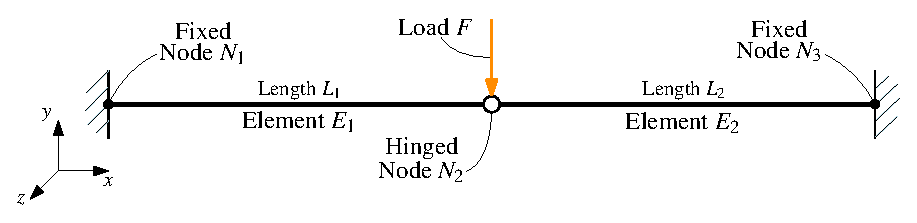
\includegraphics[width=0.7\textwidth]{./figures/appendix_4/usage_example.eps}
  \caption{Simple structure used to demonstrate the usage of the \TrussMe{} package.}
  \label{app4:fig:usage_example}
\end{figure}

To describe the structure in \TrussMe{}, we begin by defining the nodes. The \texttt{MakeNode} function is utilized for this purpose
%
\begin{verbatim}
> N1 := MakeNode("N1", <0,0,0>, dofs=<0,0,0,0,0,0>):
> N2 := MakeNode("N2", <L_1,0,0>, dofs=<1,1,1,1,1,1>):
> N3 := MakeNode("N3", <L_1+L_2,0,0>, dofs=<0,0,0,0,0,0>):
\end{verbatim}
%
This function requires the node name, coordinates, and Degrees of Freedom (\acp{DOF}) as inputs. In this case, we haven't specified reference frames, so the default ground frame (the identity matrix) is chosen for both nodes. Similarly, no constraints on displacements are specified, so they are assumed to be zero. The \acp{DOF} are set using a six-element vector. The first three elements represent displacements along the $x$-, $y$-, and $z$-axes, while the remaining three represent rotations about these axes. A value of $0$ indicates a constrained \ac{DOF}, while $1$ indicates a free \ac{DOF}. Here, nodes $N_1$ and $N_3$ are constrained in all directions, while $N_2$ is free. The hinge modeling at node $N_2$ will be explained later in this section.

Before defining the elements, the material properties must be specified. Custom materials can be defined using the \texttt{MakeMaterial} function, which requires the material name, Young's modulus, Poisson's ratio, and density as inputs. If the shear modulus isn't provided, it's calculated from Young's modulus and Poisson's ratio. In this case, the material is defined as follows.
%
\begin{verbatim}
> M := MakeMaterial(name="GenericMaterial", elastic_modulus=E, shear_modulus=G,
    poisson_ratio=nu, density=rho):
\end{verbatim}
%
Next, the \texttt{MakeBeam} function is employed, necessitating the element's name, nodes at its ends, material, and cross-section properties.
%
\begin{verbatim}
> E1 := MakeBeam("E1", N1, [N2, <0,0,0,0,0,0>], material=M, area=A, inertia=[I_x,I_y,I_z],
    frame=GenerateFrameXY(N1["coordinates"], N2["coordinates"], [0,0,1])):
> E2 := MakeBeam("E2", [N2, <0,0,0,0,0,1>], N3, material=M, area=A, inertia=[I_x,I_y,I_z],
    frame=GenerateFrameXY(N2["coordinates"], N3["coordinates"], [0,0,1])):
\end{verbatim}
%
During the element definition, the reference frame is also specified. Here, the \texttt{GenerateFrameXY} function aligns the coordinate system axes based on the coordinates of the two nodes. Additional details about how the element ends are connected to the nodes can be provided using an augmented six-element vector, such as \texttt{[N, <1,1,1,1,1,1>]}. If this vector isn't provided, the element ends are assumed to be rigidly connected to the nodes in all directions. In the provided code snippet, element $E_1$ is connected rigidly to nodes $N_1$ and $N_2$, while element $E_2$ is hinged to node $N_2$ with constrained translational \acp{DOF} and free rotational \acp{DOF}. Element $E_2$ is then rigidly connected to node $N_3$. This hinge connection is achieved by specifying the free rotational \acp{DOF} of the element ends. In this case, element $E_2$ can rotate freely around the $z$-axis.

Once the nodes and elements are defined, the loads acting on the structure can be specified using the \texttt{MakeLoad} function.
%
\begin{verbatim}
> F := MakeLoad("F", N2, <0,-P,0,0,0,0>):
\end{verbatim}
%
Similarly, the \texttt{MakeLoad} function requires the load name, the node where the load is applied, and its magnitude as inputs. Optionally, the load reference frame can be specified using the \texttt{frame} parameter. If not specified, the node's reference frame is used. In this scenario, the load is applied to node $N_2$ in the $y$-direction.

Subsequently, the \ac{FE} model of the structure can be generated using the \texttt{GenerateFEM} function, followed by solving the linear system of equations with the \texttt{SolveFEM} function.
%
\begin{verbatim}
> fem := GenerateFEM([N1,N2,N3], [E1,E2], [F], tryhard):
> SolveFEM(fem, use_LEM=false, use_LAST=false):
\end{verbatim}
%
When using the \texttt{tryhard} flag, the solvability check described in step (5b) of the list above is activated. If the \LEM{} and \LAST{} packages are preferred for solving the linear system of equations, the \texttt{use\_LEM} and \texttt{use\_LAST} flags must be set to \texttt{true}. In such cases, the solution may be obtained in a veiled form. To reveal the solution, the \texttt{use\_LEM} flag must be set to \texttt{false}. Once the linear system of equations is solved, the solution is stored in the \texttt{fem} table.
%
\begin{verbatim}
> f = fem["f"]^%T; d = fem["d"]^%T;
\end{verbatim}
\begin{equation*}
  \begin{matrix}
    f = \left[\,\begin{matrix}
      \, 0, \, \dfrac{PL_2^3}{L_1^3+L_2^3}, \, 0, \, 0, \, 0, \, \dfrac{PL_1L_2^3}{L_1^3+L_2^3}, \, 0, \, -P, \, 0, \, 0, \, 0, \, 0, \, 0, \, \dfrac{PL_1^3}{L_1^3+L_2^3}, \, 0, \, 0, \, 0, \, -\dfrac{PL_1^3L_2}{L_1^3+L_2^3} \,
    \end{matrix}\,\right] \\[1.5em]
    d = \left[\,\begin{matrix}
      \, 0, \, 0, \, 0, \, 0, \, 0, \, 0, \, 0, \, \dfrac{PL_1^3L_2^3}{3EI_z(L_1^3+L_2^3)}, \, 0, \, 0, \, 0, \, \dfrac{PL_1^2L_2^3}{2EI_z(L_1^3+L_2^3)} \, 0, \, 0, \, 0, \, 0, \, 0, \, 0 \,
    \end{matrix}\,\right]
  \end{matrix}
\end{equation*}
%
To enhance performance, the \TrussMe{} package is designed to complement the \LEM{} and \LAST{} packages, which help manage expression expansion during the symbolic solution procedure. Detailed instructions on utilizing these packages can be found in Section~\ref{chap2:sec:lem} and Section~\ref{chap2:sec:last}, as well as in their respective documentation~\cite{lem, last}. If both libraries are unavailable, the toolbox defaults to utilizing the linear algebra routines built into \Maple{}.

In cases where no symbolic solution is attainable or if the user prefers to assess the solution numerically, the \texttt{GenerateMatlabCode} function can be employed.
%
\begin{verbatim}
> GenerateMatlabCode("FemClass", fem, path="./dir/", info="Usage example class", vars=[P],
    data=[I_x=4.0e-4, I_y=2.0e-4, I_z=2.0e-4, E=210.0e6, nu=0.33, A=5.0e-3, L_1=1.0,
    L_2=1.0]);
\end{verbatim}
%
This function creates the \texttt{FemClass.m} file in the \texttt{./dir/} directory, which contains a class definition of the aforementioned \ac{FE} model. During the code generation process, users can establish default class properties in the \texttt{data} field and variable parameters in the \texttt{vars} field. The latter are intended to represent parameters that may vary during the structure analysis, such as the load magnitude $P$. Further insights into the generated class and its application are elaborated in Section~\ref{app4:subsec:numerical_computation}.

\subsection{The Numerical Computation in \Matlab{}}
\label{app4:subsec:numerical_computation}

Since the symbolic solution of~\eqref{app4:eq:macrodf} may not always be feasible, users have the option to employ a numerical solution. This involves numerically factorizing the $\mathbf{K}^{n}_{ff}$ matrix and evaluating~\eqref{app4:eq:macrosol}. The numerical solution can be achieved within the \Maple{} environment through variable substitution or in \Matlab{} post the code generation process. In the latter scenario, the \TrussMe{} \Matlab{} toolbox comes into play. This toolbox is built upon the \texttt{TrussMe.System} base class, which is utilized to define the components of~\eqref{app4:eq:macrosol} and to establish a unified framework that can be leveraged by inherited classes. Within this abstract class, various methods are present, including several virtual methods that need to be implemented in the inherited classes: \\[0.5em]
%
\begin{minipage}[t]{0.49\textwidth}
  \begin{itemize}
  \setlength{\itemsep}{-0.25em}
  \item stiffness matrix $\mathbf{K}^{n}$;
  \item free-free stiffness matrix $\mathbf{K}^{n}_{ff}$;
  \item free-specified stiffness matrix $\mathbf{K}^{n}_{fs}$;
  \item specified-free stiffness matrix $\mathbf{K}^{n}_{sf}$;
  \item specified-specified stiffness matrix $\mathbf{K}^{n}_{ss}$;
  \item displacement vector $\mathbf{d}$*;
  \item free displacement vector $\mathbf{d}^{n}_{f}$*;
  \end{itemize}
\end{minipage}
\hfill
\begin{minipage}[t]{0.49\textwidth}
  \begin{itemize}
  \setlength{\itemsep}{-0.25em}
  \item specified displacement vector $\mathbf{d}^{n}_{s}$;
  \item force vector $\mathbf{f}$*;
  \item free force vector $\mathbf{f}^{n}_{f}$;
  \item specified force vector $\mathbf{f}^{n}_{s}$*;
  \item remainder force vector $\mathbf{f}^{n}_{r}$;
  \item \acp{DOF} permutation $\mathbf{P}^{n}$;
  \item getters and setters for the system data;
  \end{itemize}
\end{minipage} \\[0.5em]
%
where (*) denotes that the functionality is accessible only when the symbolic solution of the system is available; otherwise, an empty vector is returned.

\subsubsection{Numerical Computation Usage Example}

The \TrussMe{} \Matlab{} toolbox serves to numerically assess the problem's solution. Utilizing the toolbox is straightforward, particularly when the code is generated using the \TrussMe{} \Maple{} package. Suppose we have generated the \texttt{FemClass.m} file through the \TrussMe{} \Maple{} package; this file encompasses the class definition of the structure. To employ the generated class, we first instantiate it.
%
\begin{verbatim}
>>> fem = FemClass();
\end{verbatim}
%
Optionally, during instantiation, we have the liberty to assign values to the class's internal data.
%
\begin{verbatim}
>>> data.I_x = 4.0e-4; data.I_y = 2.0e-4; data.I_z = 2.0e-4; data.E = 210.0e9; ...
    data.A = 5.0e-3; data.L_1 = 1.0; data.L_2 = 1.0;
>>> fem = FemClass(data);
\end{verbatim}
%
Following instantiation, we can manipulate the internal data values either by setting or retrieving them using dedicated methods.
%
\begin{verbatim}
>>> fem.set_data_field('I_x', 4.0e-4);
>>> I_x = fem.get_data_field('I_x');
>>> fem.set_data(data);
>>> data = fem.get_data();
\end{verbatim}
%
Once instantiated, we can acquire the components of the system of equations~\eqref{app4:eq:macrosol} through the following methods.
%
\begin{verbatim}
>>> x = [1000];
>>> v = fem.v(x);
>>> d = fem.d(x,v);
>>> f = fem.f(x,v);
\end{verbatim}
%
It's worth noting that the vector \texttt{x} encompasses the system's parameters, such as the load value $P$ of \SSI{1000}{\newton}, while the vector \texttt{v} holds the values of the veiling variables that might have been retained during the symbolic solution computation as per Section~\ref{chap2:sec:lem} and Section~\ref{chap2:sec:last}. In cases where the symbolic solution is unavailable, numerical computation becomes an alternative.
%
\begin{verbatim}
>>> x = [1000];
>>> v = fem.v(x);
>>> d = fem.compute_d(x,v);
>>> f = fem.compute_f(x,v);
\end{verbatim}
%
The least squares solution can also be acquired by incorporating the tolerance value and maximum number of iterations into the \texttt{compute\_d} and \texttt{compute\_f} methods, such as \texttt{fem.compute\_f(x,v,tol,iter)}. Alternative numerical solution methods, relying on constrained minimization of energy functional, can be utilized to solve the system of equations~\eqref{app4:eq:macrosol}~\cite{hutton2004fundamentals}. However, these methods are not currently integrated into the \TrussMe{} \Matlab{} toolbox.

% % % % % % % % % % % % % % % % % % % % % % % % % % % % % % % % % % % % % % % %

\section{Example Applications}
\label{app4:sec:example_applications}

In this section, we briefly showcase two example applications of the \TrussMe{} toolbox. All examples revolve around the rear left double wishbone suspension of the Formula SAE \emph{E-Agle Trento Racing Team} (\emph{University of Trento}) vehicle~\citep{eagle}. The suspension system is depicted in Figure~\ref{app4:fig:suspension}. On the left side, a rendering of the system is shown along with the names of its main components, while on the right side, a schematic representation of the suspension system is presented. In the subsequent paragraphs, we delve into how the \TrussMe{} toolbox can facilitate the design optimization of the suspension system and effectively incorporate the kinematics and compliance of the suspension system through model reduction. The outcomes obtained using the \TrussMe{} toolbox are validated against results obtained from the commercial software \Ansys{}. For a comprehensive analysis of the results from the example applications, please refer to~\cite{larcher2024symbolic}.

Before delving into the example applications, it's essential to clarify the workflow involving the \TrussMe{} package. In this scenario, the \TrussMe{} package is utilized to symbolically assemble the structure and simplify the expressions of its linear system components. Subsequently, the symbolic code is exported into a \Matlab{} class, where internal data and input parameters of the system are specified. This \Matlab{} class is then employed to numerically evaluate the solution of the problem within the \Simulink{} environment. This approach becomes necessary due to the significant slowdown of the symbolic kernel caused by the size and complexity of the resulting linear system.

\begin{figure}[htb]
  \centering
  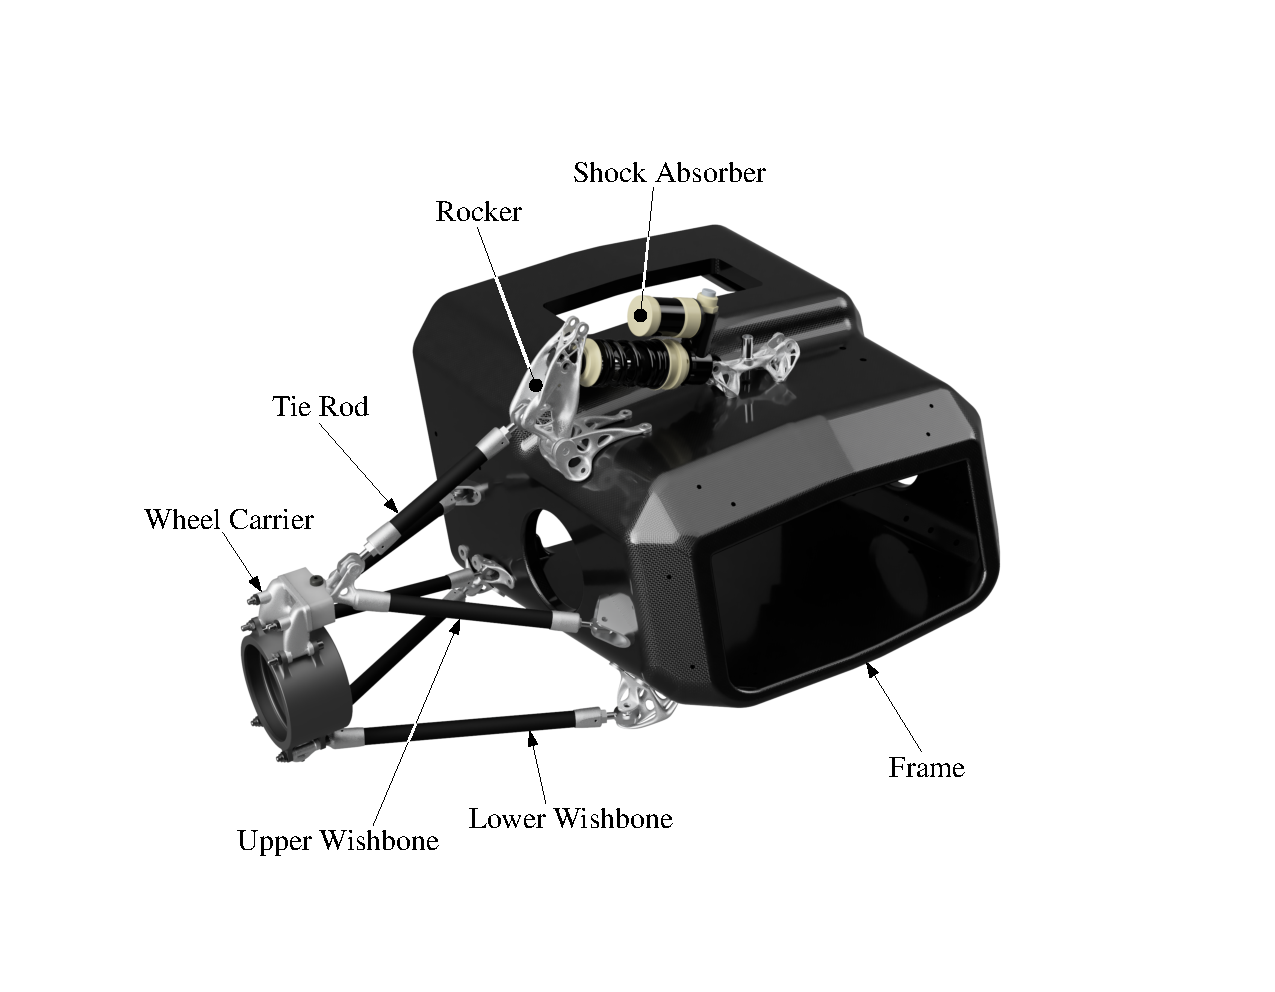
\includegraphics[width=0.5\textwidth, trim={2cm 2cm 2.5cm 2cm}, clip]{./figures/appendix_4/rendering.eps}
  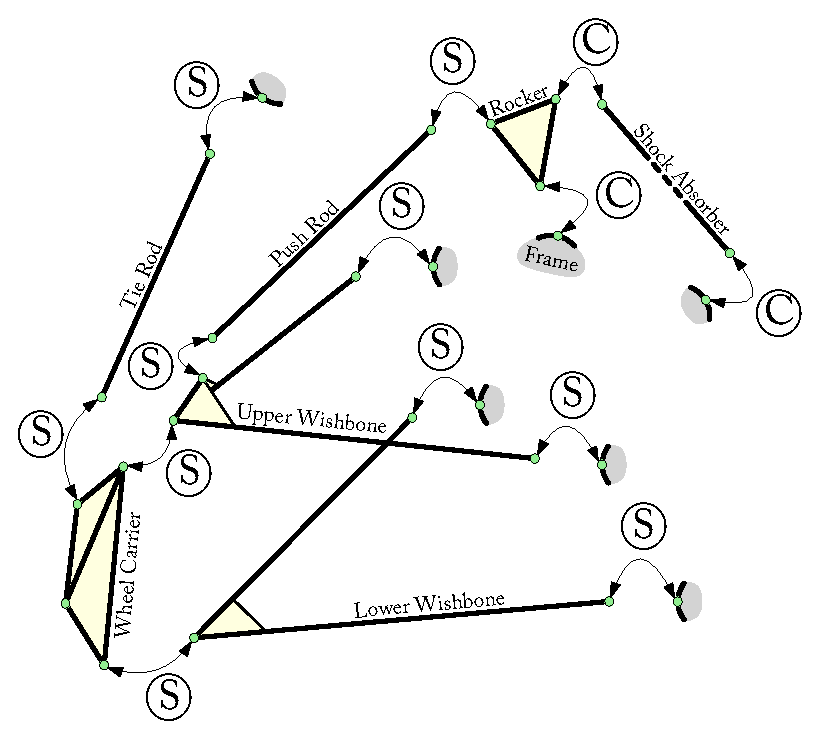
\includegraphics[width=0.4\textwidth]{./figures/appendix_4/constraints.eps}
  \caption{Rendering and schematic representation of the rear left double wishbone suspension. The spherical and cylindrical constraints are respectively represented by the symbols \circled{S} and \circled{C}.}
  \label{app4:fig:suspension}
\end{figure}

\subsection{Design Optimization}

Mechanisms involving motion are prevalent in engineering applications. Typically, the design of such mechanisms assumes rigid bodies. However, in certain instances, the flexibility of the mechanism can significantly impact its performance. Optimization emerges as a potent tool for designing structures with optimal performance. The \TrussMe{} toolbox facilitates shape optimization aimed at reducing the compliance of the mechanism and minimizing internal forces. Specifically, the presented optimizations aim to minimize both the wheel compliance hub angle $\theta_z$ and the tie rod axial force $F_a$ by varying the $x$- and $z$- coordinates of the hard point connecting the tie rod to the chassis, referred to as point $P_5$ according to~\cite{larcher2024symbolic}. The results of these optimizations are depicted in Figure~\ref{app4:fig:optimization}. These optimization demonstrations underscore that the current design does not represent the optimal solution in terms of minimum tie rod axial force and minimum wheel compliance hub angle. Optimum conditions are attained through a combination of values indicated by the green point. It's noteworthy that these optimization examples serve solely as a proof of concept for the model's parametric characteristics. In a real-world scenario, a multi-objective optimization considering compliance, structural analysis, and kinematic characteristics of the suspension would be imperative.

\begin{figure}[htb]
  \centering
    \begin{subfigure}[t]{0.49\textwidth}
    \small{\includetikz{figures/appendix_4/optimization_hub_angle.tex}}
    \caption{Wheel hub compliance angle $\theta_z$ dependency from the $x$- and $z$- coordinates of the $P_5$ hard point.}
    \label{app4:fig:variation_theta_z}
  \end{subfigure}
  \hfill
  \begin{subfigure}[t]{0.49\textwidth}
    \centering
    \small{\includetikz{figures/appendix_4/optimization_tie_force.tex}}
    \caption{Tie rod axial force $F_a$ dependency from the $x$- and $z$- coordinates of the $P_5$ hard point.}
    \label{app4:fig:variation_force_tie}
  \end{subfigure}
  \caption{Optimization is conducted on the coordinates of point $P_5$, specifically its $x$- and $z$-coordinates, with the aim of minimizing both the wheel compliance hub angle $\theta_z$ and the tie rod axial force $F_a$. The experiments are conducted under the application of a constant torque $M_z$ of \SI{0.4}{\kilo\newton\meter}. \emph{Marks legend:} {\color{mycolor2}\raisebox{-.15pt}{\Large$\bullet$}} current design, {\color{mycolor5}\raisebox{-.15pt}{\Large$\bullet$}} optimality condition.}
  \label{app4:fig:optimization}
\end{figure}

\begin{figure}[htp!]
  \centering
  \small{\includetikz{figures/appendix_4/suspension_static_deformations.tex}}
  \caption{The figure illustrates a comparison of displacements and rotations of the wheel carrier reference frame about the $x$-, $y$-, and $z$-axes for various loads applied at the wheel hub. The results are obtained using both the \TrussMe{} toolbox (\emph{lines}) and the \Ansys{} finite element analysis software (\emph{dots}). On the left-hand side of the figure, forces are applied while torques are null, whereas on the right-hand side, torques are applied while forces are null.}
  \label{app4:fig:suspension_static_results}
\end{figure}

\subsection{Efficient Simulation of Parametric Mechanisms Using Model Reduction}

This example application explores the inclusion of suspension compliance in vehicle simulation using a hybrid symbolic-numerical approach. This methodology facilitates easy generalization and real-time modification of model parameters without the need for code regeneration. The suspension's dynamic characteristics are modeled through a system of differential-algebraic equations, integrated using methods described in~\cite{larcher2024symbolic}. Depending on the modeling approach, suspension pick-up points' positions and tire force at the hub are extracted either through semi-analytical solutions or numerical integration. These are then utilized to calculate the suspension's compliance characteristics. The compliance contribution can be incorporated into the overall suspension system displacement as either a \emph{steady-state} or \emph{full dynamic} contribution~\cite{larcher2024symbolic}. The former approach reduces computational costs, while the latter yields accurate simulations at a higher computational expense. Results from this approach are compared with simulation data from commercial software \Ansys{}, showing good agreement under both static (\figurename{}~\ref{app4:fig:suspension_static_results}) and dynamic conditions (\figurename{}~\ref{chap4:fig:suspension_dynamic_results}).

% % % % % % % % % % % % % % % % % % % % % % % % % % % % % % % % % % % % % % % %

%\section{Conclusions}
%\label{app4:sec:conclusion}

%This chapter introduces the \TrussMe{} toolbox, a symbolic-numerical toolbox for structural analysis. Based on the \ac{DSM}, it proves valuable for modeling, simulating, and optimizing structures. The toolbox comprises two parts: a symbolic manipulation component implemented as a \Maple{} package, responsible for assembling and simplifying linear systems of equations. Symbolic code is exported to a \Matlab{} class via code generation. The numerical component, implemented in \Matlab{}, evaluates the problem solution numerically if a symbolic solution is unavailable. Validation of the \TrussMe{} toolbox is demonstrated through two example applications. Additionally, difficulties in computing the symbolic solution of linear systems are mitigated by optional tools like \LEM{}\cite{lem} and \LAST{}\cite{last} \Maple{} packages, which are presented for use alongside the \TrussMe{} toolbox.

% % % % % % % % % % % % % % % % % % % % % % % % % % % % % % % % % % % % % % % %
